\documentclass[11pt,a4paper]{article}

% ── Packages ──────────────────────────────────────────────────────────
\usepackage[utf8]{inputenc}
\usepackage[T1]{fontenc}
\usepackage{lmodern}
\usepackage[margin=2.4cm]{geometry}
\usepackage{amsmath,amssymb}
\usepackage{booktabs}
\usepackage{array}
\usepackage{longtable}
\usepackage{graphicx}
\usepackage{xcolor}
\usepackage{hyperref}
\usepackage{enumitem}
\usepackage{fancyhdr}
\usepackage{titlesec}
\usepackage{float}
\usepackage{caption}
\usepackage{multicol}
\usepackage{multirow}
\usepackage{tikz}
\usepackage{pgfplots}
\pgfplotsset{compat=1.18}
\usetikzlibrary{arrows.meta,positioning,calc,fit,shapes.geometric,backgrounds}

\hypersetup{
    colorlinks=true,
    linkcolor=blue!70!black,
    citecolor=green!50!black,
    urlcolor=blue!60!black,
}

\pagestyle{fancy}
\fancyhf{}
\fancyhead[L]{\small\textit{EigenDialectos --- Software Architecture Report}}
\fancyhead[R]{\small\thepage}
\renewcommand{\headrulewidth}{0.4pt}

\titleformat{\section}{\Large\bfseries\color{blue!70!black}}{}{0em}{}
\titleformat{\subsection}{\large\bfseries\color{blue!50!black}}{}{0em}{}
\titleformat{\subsubsection}{\normalsize\bfseries\color{blue!30!black}}{}{0em}{}

\definecolor{eigen3col}{RGB}{50,120,200}
\definecolor{edcol}{RGB}{180,60,60}
\definecolor{scriptcol}{RGB}{60,160,60}
\definecolor{testcol}{RGB}{160,120,40}
\definecolor{layercol1}{RGB}{230,245,255}
\definecolor{layercol2}{RGB}{255,235,230}
\definecolor{layercol3}{RGB}{235,255,235}
\definecolor{layercol4}{RGB}{255,250,230}
\definecolor{layercol5}{RGB}{240,235,255}

% ── Document ──────────────────────────────────────────────────────────
\begin{document}

\begin{titlepage}
\centering
\vspace*{3cm}
{\Huge\bfseries\color{blue!70!black} EigenDialectos\\[0.3em]
Software Architecture Report\par}
\vspace{1.5cm}
{\Large Codebase Structure, Module Inventory,\\
and Lines-of-Code Analysis\par}
\vspace{2cm}
{\large
\begin{tabular}{rl}
\textbf{Project:} & EigenDialectos --- Spanish Dialect Spectral Geometry \\
\textbf{Date:} & April 10, 2026 \\
\textbf{Total Python files:} & 319 \\
\textbf{Total LOC:} & 79{,}325 \\
\textbf{Test files:} & 63 (14{,}874 LOC) \\
\textbf{Test/source ratio:} & 23\% \\
\end{tabular}
\par}
\vspace{3cm}
{\small\textit{Internal technical report --- EigenDialectos research pipeline}}
\end{titlepage}

\tableofcontents
\newpage

% ══════════════════════════════════════════════════════════════════════
\section{Executive Summary}
% ══════════════════════════════════════════════════════════════════════

EigenDialectos is a research system for computing and analyzing spectral
representations of Spanish dialect variation. It processes raw text corpora from
8~Spanish varieties into per-variety word embeddings, decomposes the
variety-to-variety transformation matrices via eigenanalysis, and uses the resulting
spectral features for dialect classification, generation, interpolation, and
geometric analysis.

The codebase comprises \textbf{79{,}325 lines of Python} across \textbf{319 files},
organized into four major layers:

\begin{enumerate}[nosep]
  \item \textbf{\texttt{eigen3}} (13{,}034 LOC, 36 files) --- The v3 core:
        transformer training, spectral algebra, downstream experiments.
  \item \textbf{\texttt{eigendialectos}} (42{,}035 LOC, 201 files) --- The v2
        expanded codebase: corpus acquisition, multi-method embeddings, compiler,
        generative models, validation.
  \item \textbf{\texttt{scripts}} (9{,}382 LOC, 21 files) --- Pipeline runners,
        analysis scripts, corpus tools.
  \item \textbf{\texttt{tests}} (14{,}874 LOC, 63 files) --- Unit, integration,
        and property-based tests.
\end{enumerate}

\begin{figure}[H]
\centering
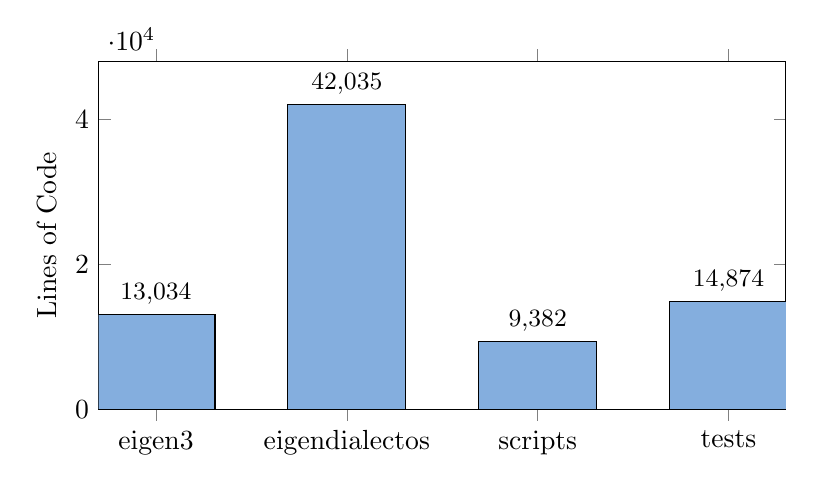
\begin{tikzpicture}
\begin{axis}[
    ybar,
    width=0.85\textwidth,
    height=6cm,
    ylabel={Lines of Code},
    symbolic x coords={eigen3, eigendialectos, scripts, tests},
    xtick=data,
    nodes near coords,
    nodes near coords style={font=\small},
    ymin=0, ymax=48000,
    bar width=1.5cm,
    every node near coord/.append style={anchor=south},
]
\addplot[fill=eigen3col!60] coordinates {
    (eigen3,13034) (eigendialectos,42035) (scripts,9382) (tests,14874)
};
\end{axis}
\end{tikzpicture}
\caption{Lines of code by top-level module.}
\end{figure}


% ══════════════════════════════════════════════════════════════════════
\section{High-Level Architecture}
% ══════════════════════════════════════════════════════════════════════

\subsection{System Pipeline}

The end-to-end pipeline follows a five-stage dataflow:

\begin{figure}[H]
\centering
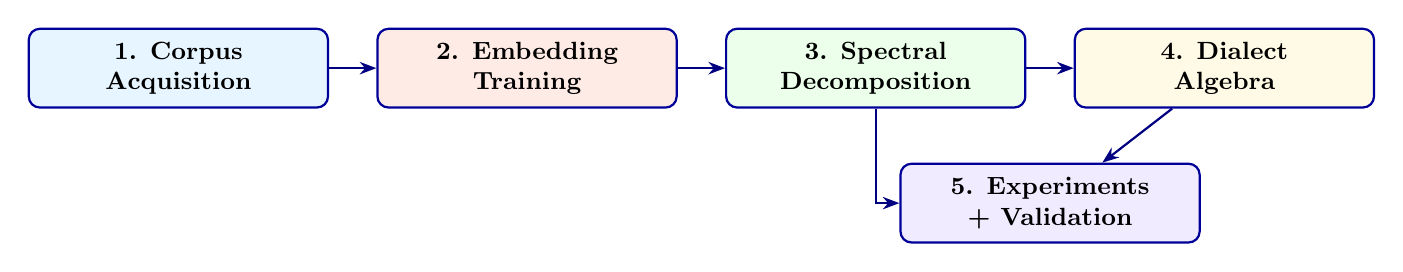
\begin{tikzpicture}[
    node distance=0.6cm,
    stage/.style={
        rectangle, rounded corners=4pt, draw=blue!60!black, thick,
        minimum width=3.8cm, minimum height=1.0cm, align=center,
        font=\small\bfseries
    },
    arrow/.style={-{Stealth[length=6pt]}, thick, blue!50!black}
]
\node[stage, fill=layercol1] (corpus) {1. Corpus\\Acquisition};
\node[stage, fill=layercol2, right=of corpus] (embed) {2. Embedding\\Training};
\node[stage, fill=layercol3, right=of embed] (spectral) {3. Spectral\\Decomposition};
\node[stage, fill=layercol4, right=of spectral] (algebra) {4. Dialect\\Algebra};
\node[stage, fill=layercol5, below=1.2cm of $(spectral)!0.5!(algebra)$] (exp) {5. Experiments\\+ Validation};

\draw[arrow] (corpus) -- (embed);
\draw[arrow] (embed) -- (spectral);
\draw[arrow] (spectral) -- (algebra);
\draw[arrow] (algebra) -- (exp);
\draw[arrow] (spectral) |- (exp);
\end{tikzpicture}
\caption{Pipeline stages. Each stage has dedicated modules in both \texttt{eigen3} and \texttt{eigendialectos}.}
\end{figure}

\begin{description}[style=nextline,leftmargin=2em]
  \item[Stage 1: Corpus Acquisition]
    Web scraping, API downloads (Reddit, OpenSubtitles, Wikipedia, lyrics),
    synthetic augmentation, balancing, and preprocessing. Input: URLs and API keys.
    Output: per-variety JSONL files.

  \item[Stage 2: Embedding Training]
    Two methods: (a)~BETO + LoRA transformer with SupCon contrastive training;
    (b)~legacy BPE + skip-gram with DCL. Input: balanced corpus. Output: per-variety
    word embedding matrices $E_v \in \mathbb{R}^{V \times d}$.

  \item[Stage 3: Spectral Decomposition]
    Procrustes alignment to reference variety (ES\_PEN), computation of
    transformation matrices $W_{v \to u}$, eigendecomposition, residual analysis.
    Output: eigenvalues, eigenvectors, spectral features per variety pair.

  \item[Stage 4: Dialect Algebra]
    Composition, interpolation, analogy, and arithmetic on spectral representations.
    Dialect generation via eigenmode manipulation. Output: synthetic spectra,
    interpolated embeddings, Fisher diagnostic words.

  \item[Stage 5: Experiments + Validation]
    15 defined experiments (spectral maps, phase transitions, impossible dialects,
    cross-linguistic transfer, etc.) plus quantitative (classification, perplexity,
    holdout) and qualitative (Turing test, survey, HYPERDIA) validation.
\end{description}


\subsection{Module Dependency Architecture}

\begin{figure}[H]
\centering
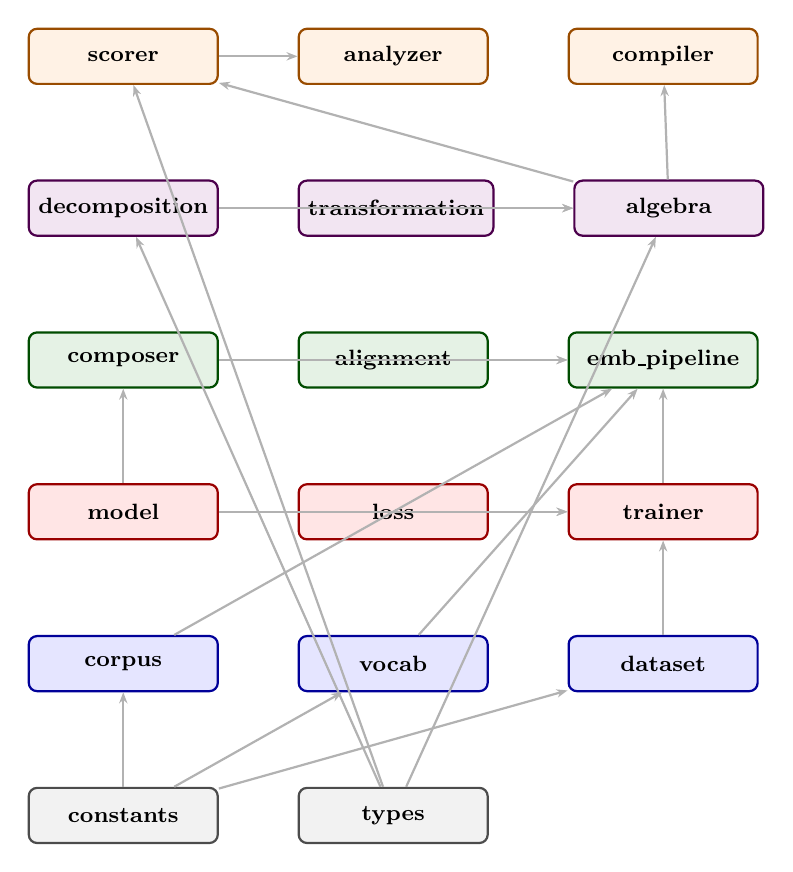
\begin{tikzpicture}[
    node distance=0.8cm and 1.0cm,
    mod/.style={
        rectangle, rounded corners=3pt, draw=#1!60!black, thick,
        fill=#1!10, minimum width=2.4cm, minimum height=0.7cm,
        align=center, font=\footnotesize\bfseries
    },
    arr/.style={-{Stealth[length=4pt]}, thick, gray!60},
]
% Layer 0: Constants / Types
\node[mod=gray] (const) {constants};
\node[mod=gray, right=of const] (types) {types};

% Layer 1: Data
\node[mod=blue, above=1.2cm of const] (corpus) {corpus};
\node[mod=blue, right=of corpus] (vocab) {vocab};
\node[mod=blue, right=of vocab] (dataset) {dataset};

% Layer 2: Model
\node[mod=red, above=1.2cm of corpus] (model) {model};
\node[mod=red, right=of model] (loss) {loss};
\node[mod=red, right=of loss] (trainer) {trainer};

% Layer 3: Extraction
\node[mod=green!50!black, above=1.2cm of model] (composer) {composer};
\node[mod=green!50!black, right=of composer] (alignment) {alignment};
\node[mod=green!50!black, right=of alignment] (pipeline) {emb\_pipeline};

% Layer 4: Analysis
\node[mod=violet, above=1.2cm of composer] (decomp) {decomposition};
\node[mod=violet, right=of decomp] (transform) {transformation};
\node[mod=violet, right=of transform] (algebra) {algebra};

% Layer 5: Applications
\node[mod=orange, above=1.2cm of decomp] (scorer) {scorer};
\node[mod=orange, right=of scorer] (analyzer) {analyzer};
\node[mod=orange, right=of analyzer] (compiler) {compiler};

% Arrows (simplified)
\draw[arr] (const) -- (corpus);
\draw[arr] (const) -- (vocab);
\draw[arr] (const) -- (dataset);
\draw[arr] (types) -- (decomp);
\draw[arr] (types) -- (algebra);
\draw[arr] (types) -- (scorer);
\draw[arr] (corpus) -- (pipeline);
\draw[arr] (vocab) -- (pipeline);
\draw[arr] (dataset) -- (trainer);
\draw[arr] (model) -- (trainer);
\draw[arr] (model) -- (composer);
\draw[arr] (loss) -- (trainer);
\draw[arr] (trainer) -- (pipeline);
\draw[arr] (composer) -- (pipeline);
\draw[arr] (alignment) -- (pipeline);
\draw[arr] (decomp) -- (algebra);
\draw[arr] (transform) -- (algebra);
\draw[arr] (algebra) -- (compiler);
\draw[arr] (algebra) -- (scorer);
\draw[arr] (scorer) -- (analyzer);
\end{tikzpicture}
\caption{Dependency graph of \texttt{eigen3} core modules (simplified). Arrows point from dependency to dependent.}
\end{figure}


% ══════════════════════════════════════════════════════════════════════
\section{Module Inventory: \texttt{src/eigen3/}}
% ══════════════════════════════════════════════════════════════════════

The \texttt{eigen3} package contains 36 Python files totaling 13{,}034 LOC. This is
the active codebase for the v3 transformer pipeline.

\subsection{LOC Breakdown by File}

\begin{longtable}{@{}rlrl@{}}
\toprule
\textbf{Rank} & \textbf{File} & \textbf{LOC} & \textbf{Category} \\
\midrule
\endhead
1 & \texttt{downloader\_v45.py} & 1{,}057 & Data acquisition \\
2 & \texttt{scraper.py} & 1{,}053 & Data acquisition \\
3 & \texttt{downloader.py} & 998 & Data acquisition \\
4 & \texttt{constants.py} & 808 & Configuration \\
5 & \texttt{analyzer.py} & 747 & Spectral analysis \\
6 & \texttt{trainer.py} & 743 & Training loop \\
7 & \texttt{corpus.py} & 665 & Corpus processing \\
8 & \texttt{algebra.py} & 639 & Spectral algebra \\
9 & \texttt{scorer.py} & 608 & Dialect scoring \\
10 & \texttt{compiler.py} & 500 & SDC compilation \\
11 & \texttt{dataset.py} & 367 & Data loading \\
12 & \texttt{residual.py} & 344 & Residual analysis \\
13 & \texttt{emb\_pipeline.py} & 341 & Pipeline orchestration \\
14 & \texttt{per\_mode.py} & 339 & Eigenmode ops \\
15 & \texttt{model.py} & 338 & Neural architecture \\
16 & \texttt{probing.py} & 329 & Probing tasks \\
17 & \texttt{validation.py} & 306 & Validation metrics \\
18 & \texttt{topology.py} & 277 & Persistent homology \\
19 & \texttt{vocab.py} & 272 & Vocabulary mgmt \\
20 & \texttt{loss.py} & 249 & Loss functions \\
21 & \texttt{eigenfield.py} & 239 & Eigenvalue fields \\
22 & \texttt{lie.py} & 229 & Lie algebra \\
23 & \texttt{composer.py} & 218 & Embedding extraction \\
24 & \texttt{fisher.py} & 215 & Fisher information \\
25 & \texttt{riemannian.py} & 195 & Riemannian geometry \\
26 & \texttt{types.py} & 161 & Type definitions \\
27 & \texttt{core.py} & 122 & Public API \\
28 & \texttt{multigranularity.py} & 101 & Multi-scale decomp \\
29 & \texttt{tokenizer.py} & 100 & BPE tokenizer \\
30 & \texttt{distance.py} & 79 & Distance metrics \\
31 & \texttt{alignment.py} & 79 & Procrustes alignment \\
32 & \texttt{null\_model.py} & 75 & Null baseline \\
33 & \texttt{transformation.py} & 74 & $W$ matrices \\
34 & \texttt{decomposition.py} & 72 & Eigendecomposition \\
35 & \texttt{stability.py} & 52 & Numerical stability \\
36 & \texttt{\_\_init\_\_.py} & 43 & Package init \\
\midrule
& \textbf{Total} & \textbf{13{,}034} & \\
\bottomrule
\end{longtable}

\subsection{Functional Grouping}

\begin{table}[H]
\centering
\caption{Eigen3 files grouped by functional layer.}
\begin{tabular}{@{}llr@{}}
\toprule
\textbf{Layer} & \textbf{Files} & \textbf{LOC} \\
\midrule
Data acquisition & downloader\_v45, scraper, downloader & 3{,}108 \\
Corpus \& vocabulary & corpus, vocab, constants, types & 1{,}906 \\
Training pipeline & model, loss, dataset, trainer, tokenizer & 1{,}797 \\
Embedding extraction & composer, alignment, emb\_pipeline & 638 \\
Spectral analysis & decomposition, transformation, algebra, per\_mode & 1{,}124 \\
Downstream analysis & scorer, analyzer, compiler, residual, probing & 2{,}528 \\
Geometry \& topology & riemannian, lie, fisher, eigenfield, topology & 1{,}155 \\
Utilities & core, distance, null\_model, stability, multigranularity & 429 \\
\bottomrule
\end{tabular}
\end{table}

\subsection{Class Inventory}

\begin{table}[H]
\centering
\caption{Major classes defined in \texttt{eigen3}.}
\small
\begin{tabular}{@{}llrl@{}}
\toprule
\textbf{Class} & \textbf{File} & \textbf{LOC} & \textbf{Purpose} \\
\midrule
\texttt{DialectTransformer} & model.py & $\sim$150 & BETO + LoRA + variety tokens \\
\texttt{DialectAttentionPooling} & model.py & $\sim$30 & Learned attention pooling \\
\texttt{DCLModel} & model.py & $\sim$50 & Legacy skip-gram model \\
\texttt{DialectMultiTaskLoss} & loss.py & $\sim$130 & MLM + CLS + SupCon loss \\
\texttt{DialectContrastiveLoss} & loss.py & $\sim$30 & Legacy DCL loss \\
\texttt{TransformerTrainer} & trainer.py & $\sim$450 & Training loop + XBM + logging \\
\texttt{DCLTrainer} & trainer.py & $\sim$200 & Legacy skip-gram trainer \\
\texttt{DialectMLMDataset} & dataset.py & $\sim$120 & MLM + variety-labeled dataset \\
\texttt{BalancedVarietySampler} & dataset.py & $\sim$50 & $k$-per-variety batch sampler \\
\texttt{TransformerWordComposer} & composer.py & $\sim$130 & Contextual $\to$ static extraction \\
\texttt{EigenDialectos} & core.py & $\sim$80 & Public API facade \\
\texttt{DialectScorer} & scorer.py & $\sim$400 & Multi-metric scoring \\
\texttt{EigenvalueField} & eigenfield.py & $\sim$150 & Continuous eigenvalue fields \\
\texttt{Tokenizer} & tokenizer.py & $\sim$60 & BPE tokenizer wrapper \\
\bottomrule
\end{tabular}
\end{table}


% ══════════════════════════════════════════════════════════════════════
\section{Module Inventory: \texttt{src/eigendialectos/}}
% ══════════════════════════════════════════════════════════════════════

The \texttt{eigendialectos} package is the v2 expanded codebase: 201 files, 42{,}035 LOC.
It provides modular, pluggable implementations for each pipeline stage.

\subsection{Sub-package Breakdown}

\begin{table}[H]
\centering
\caption{Eigendialectos sub-packages.}
\begin{tabular}{@{}lrrp{7cm}@{}}
\toprule
\textbf{Sub-package} & \textbf{Files} & \textbf{LOC} & \textbf{Description} \\
\midrule
\texttt{corpus/} & 22 & 9{,}842 & Acquisition (web, API, synthetic), parsing (phrase, morpheme, discourse), preprocessing (labeling, filters, balancing, noise, segmentation) \\
\texttt{embeddings/} & 29 & 5{,}748 & 6 embedding families: DCL, contrastive alignment, sentence (BETO/MARIa/SpanBERT), subword (BPE/FastText), word (GloVe/Word2Vec), plus pipeline \& registry \\
\texttt{experiments/} & 15 & 4{,}625 & 13 defined experiments: spectral maps, phase transitions, impossible dialects, cross-linguistic, eigenvalue archaeology, synthetic dialect, code-switching, etc. \\
\texttt{spectral/} & 11 & 2{,}698 & Decomposition, distance, eigenvector analysis, null model, multigranularity, entropy, transformation, stack \\
\texttt{validation/} & 10 & 1{,}639 & Quantitative (classification, perplexity, holdout) and qualitative (Turing test, survey, HYPERDIA) \\
\texttt{compiler/} & 5 & 1{,}263 & SDC transformer, residual, reconstructor, parser \\
\texttt{cli/} & 6 & 1{,}154 & Click-based CLI: spectral, embedding, corpus, generate, experiment commands \\
\texttt{generative/} & 6 & 1{,}048 & Dialect generation, LoRA integration, intensity, mixing, constraints \\
\texttt{algebra/} & 6 & 975 & Model + domain-specific: lexical, morphosyntactic, phonological, pragmatic, regionalism \\
\texttt{geometry/} & 4 & 846 & Eigenvalue fields, Riemannian manifolds, Lie algebra, Fisher information \\
\texttt{tensor/} & 5 & 747 & CP/Tucker decomposition, construction, analysis, visualization \\
\texttt{utils/} & 5 & 673 & I/O, logging, reproducibility, GPU, checkpointing \\
\texttt{topology/} & 1 & 313 & Persistent homology, Betti numbers, persistence entropy \\
\texttt{visualization/} & 7 & --- & Dialect maps, embedding/spectral/gradient/tensor plots \\
\midrule
& \textbf{201} & \textbf{42{,}035} & \\
\bottomrule
\end{tabular}
\end{table}

\subsection{Top 20 Largest Files}

\begin{longtable}{@{}rllr@{}}
\toprule
\textbf{Rank} & \textbf{Sub-package} & \textbf{File} & \textbf{LOC} \\
\midrule
\endhead
1 & corpus/synthetic & enhanced\_synthetic.py & 2{,}426 \\
2 & embeddings/dcl & llm\_regionalisms.py & 1{,}351 \\
3 & corpus/acquisition & web\_scraper.py & 1{,}240 \\
4 & export & exporter.py & 1{,}065 \\
5 & corpus/acquisition & lyrics\_fetcher.py & 1{,}007 \\
6 & corpus/acquisition & reddit\_fetcher.py & 816 \\
7 & corpus/acquisition & opensubtitles\_fetcher.py & 761 \\
8 & corpus/acquisition & wikipedia\_fetcher.py & 696 \\
9 & embeddings & pipeline.py & 578 \\
10 & experiments & exp\_g\_cross\_linguistic.py & 574 \\
11 & corpus/synthetic & templates.py & 567 \\
12 & embeddings/dcl & trainer.py & 556 \\
13 & corpus/parsing & phrase\_parser.py & 544 \\
14 & corpus/parsing & morpheme\_parser.py & 517 \\
15 & experiments & exp\_d\_synthetic\_dialect.py & 483 \\
16 & embeddings & vocab\_filter.py & 456 \\
17 & spectral & residual\_analysis.py & 450 \\
18 & compiler & transformer.py & 436 \\
19 & corpus/parsing & discourse\_parser.py & 423 \\
20 & corpus/synthetic & fixtures.py & 417 \\
\bottomrule
\end{longtable}


% ══════════════════════════════════════════════════════════════════════
\section{Scripts Layer}
% ══════════════════════════════════════════════════════════════════════

21 scripts totaling 9{,}382 LOC serve as entry points for pipeline execution,
analysis, and validation.

\begin{table}[H]
\centering
\caption{Scripts by function.}
\small
\begin{tabular}{@{}llrl@{}}
\toprule
\textbf{Category} & \textbf{Script} & \textbf{LOC} & \textbf{Purpose} \\
\midrule
\multirow{3}{*}{\textbf{Training}} & train\_eigen3.py & 179 & v3 transformer training \\
 & run\_pipeline.py & 1{,}190 & Full pipeline runner \\
 & run\_pipeline\_v2.py & 488 & v2 pipeline runner \\
 & full\_pipeline.py & 291 & End-to-end pipeline \\
\midrule
\multirow{3}{*}{\textbf{Data}} & build\_corpus.py & 503 & Corpus construction \\
 & download\_corpus\_v4.py & 102 & v4 corpus download \\
 & download\_v45\_source.py & 83 & v4.5 source download \\
 & merge\_v45\_corpus.py & 207 & Corpus merging \\
\midrule
\multirow{4}{*}{\textbf{Analysis}} & run\_analysis.py & 138 & Analysis runner \\
 & analyze\_results.py & 964 & Results analysis \\
 & compare\_methods.py & 578 & Method comparison \\
 & bootstrap\_ci.py & 459 & Confidence intervals \\
 & linguistic\_categorization.py & 449 & Linguistic analysis \\
 & corpus\_balance\_sensitivity.py & 405 & Balance sensitivity \\
 & baseline\_comparison.py & 361 & Baseline comparison \\
\midrule
\multirow{4}{*}{\textbf{Validation}} & validate\_v2\_comprehensive.py & 1{,}279 & v2 full validation \\
 & validate\_project.py & 769 & Project validation \\
 & validate\_v3\_full.py & 233 & v3 validation \\
 & run\_v2\_real.py & 645 & v2 real-data run \\
\midrule
\textbf{Report} & generate\_report.py & 59 & Report generation \\
\bottomrule
\end{tabular}
\end{table}


% ══════════════════════════════════════════════════════════════════════
\section{Test Suite}
% ══════════════════════════════════════════════════════════════════════

63 test files (including 2 conftest.py) totaling 14{,}874 LOC provide coverage
across all pipeline stages. The test-to-source ratio is 23\%.

\subsection{Test Distribution}

\begin{table}[H]
\centering
\caption{Test suite breakdown.}
\begin{tabular}{@{}lrrp{5.5cm}@{}}
\toprule
\textbf{Category} & \textbf{Files} & \textbf{LOC} & \textbf{Key Areas} \\
\midrule
\texttt{test\_eigen3/} & 14 & 5{,}930 & Scorer accuracy (808), dialect arithmetic (567), SDC compiler (559), dialect scoring (548), continuous dialectalization (533), eigenmode linguistics (493) \\
\texttt{test\_corpus/} & 4 & 1{,}254 & Preprocessing, sources, dataset, synthetic \\
\texttt{test\_embeddings/} & 5 & 1{,}189 & Contrastive, word, alignment, subword, sentence \\
\texttt{test\_spectral/} & 4 & 903 & Distance, transformation, decomposition, entropy \\
\texttt{test\_generative/} & 4 & 715 & DIAL, generator, intensity, mixing \\
\texttt{test\_experiments/} & 8 & 891 & All 7 experiment types + conftest \\
\texttt{test\_v2/} & 5 & 672 & Geometry, spectral stack, DCL, parsing, topology \\
\texttt{test\_validation/} & 2 & 667 & Quantitative (406), qualitative (261) \\
\texttt{test\_visualization/} & 1 & 467 & All plot types \\
\texttt{test\_tensor/} & 3 & 374 & CP, Tucker, construction \\
\texttt{test\_algebra/} & 1 & 260 & Algebraic model \\
\texttt{integration/} & 4 & 308 & 4 end-to-end pipelines \\
\texttt{conftest.py} & 2 & 244 & Fixtures and configuration \\
\midrule
\textbf{Total} & \textbf{63} & \textbf{14{,}874} & \\
\bottomrule
\end{tabular}
\end{table}

\subsection{Test Coverage Characteristics}

\begin{itemize}[nosep]
  \item \textbf{Strongest coverage:} Spectral algebra, scoring, SDC compiler,
        eigenmode analysis (test\_eigen3 alone is 5{,}930 LOC).
  \item \textbf{No unit tests for:} v2 transformer training loop
        (\texttt{TransformerTrainer}), SupCon loss (\texttt{DialectMultiTaskLoss}),
        balanced sampler (\texttt{BalancedVarietySampler}), XBM queue mechanics.
        These components were tested via end-to-end smoke runs.
  \item \textbf{Integration tests:} 4 tests covering corpus$\to$embedding,
        embedding$\to$spectral, spectral$\to$generative, and full pipeline.
  \item All 742 tests pass on the current v2 codebase (verified April 9, 2026).
\end{itemize}


% ══════════════════════════════════════════════════════════════════════
\section{External Dependencies}
% ══════════════════════════════════════════════════════════════════════

\begin{table}[H]
\centering
\caption{Third-party dependencies by category.}
\small
\begin{tabular}{@{}lp{10cm}@{}}
\toprule
\textbf{Category} & \textbf{Packages} \\
\midrule
Scientific computing & \texttt{numpy}, \texttt{scipy} (linalg, stats, spatial, cluster), \texttt{scikit-learn} (decomposition, manifold), \texttt{pandas} \\
Deep learning & \texttt{torch} (nn, optim, cuda), \texttt{transformers} (HuggingFace), \texttt{peft} (LoRA) \\
NLP & \texttt{spacy}, \texttt{sentencepiece}, \texttt{gensim}, \texttt{fasttext} \\
Visualization & \texttt{matplotlib}, \texttt{seaborn}, \texttt{plotly} \\
Web / data & \texttt{requests}, \texttt{beautifulsoup4}, \texttt{urllib} \\
CLI & \texttt{click} \\
Config / serialization & \texttt{pyyaml}, \texttt{json}, \texttt{pickle} \\
\bottomrule
\end{tabular}
\end{table}


% ══════════════════════════════════════════════════════════════════════
\section{Training Subsystem Deep Dive}
% ══════════════════════════════════════════════════════════════════════

The training subsystem is the most complex component and the focus of the
current v2 work. It spans 6 files in \texttt{eigen3/} totaling 2{,}256 LOC.

\subsection{Training Pipeline Architecture}

\begin{figure}[H]
\centering
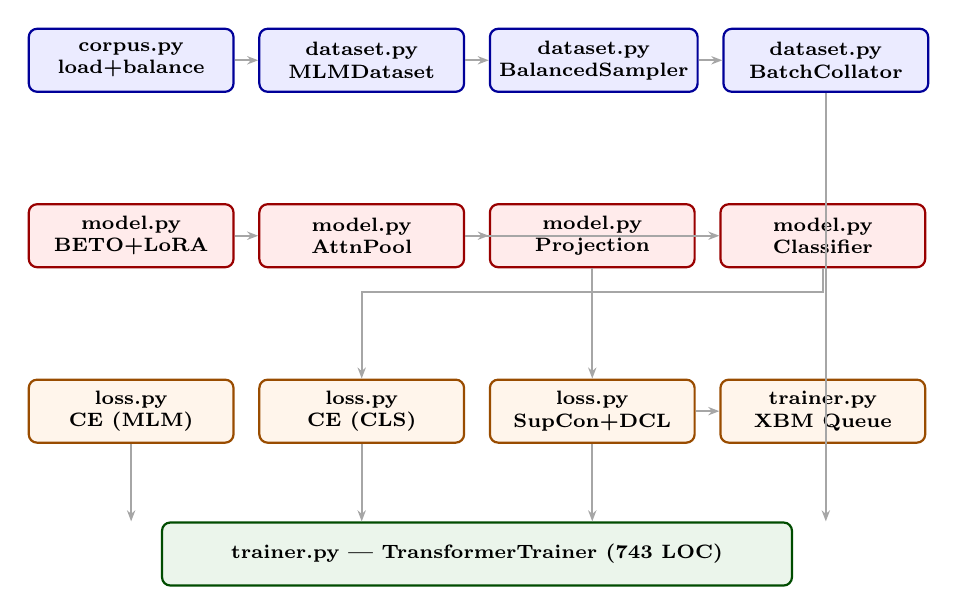
\begin{tikzpicture}[
    node distance=0.5cm and 0.3cm,
    comp/.style={
        rectangle, rounded corners=3pt, draw=#1!60!black,
        fill=#1!8, minimum width=2.6cm, minimum height=0.8cm,
        align=center, font=\scriptsize\bfseries, thick
    },
    data/.style={comp=blue},
    model/.style={comp=red},
    loss/.style={comp=orange},
    flow/.style={-{Stealth[length=4pt]}, thick, gray!70},
]
% Data path
\node[data] (corpus) {corpus.py\\load+balance};
\node[data, right=of corpus] (dataset) {dataset.py\\MLMDataset};
\node[data, right=of dataset] (sampler) {dataset.py\\BalancedSampler};
\node[data, right=of sampler] (collator) {dataset.py\\BatchCollator};

% Model path
\node[model, below=1.4cm of corpus] (beto) {model.py\\BETO+LoRA};
\node[model, right=of beto] (pool) {model.py\\AttnPool};
\node[model, right=of pool] (proj) {model.py\\Projection};
\node[model, right=of proj] (cls) {model.py\\Classifier};

% Loss path
\node[loss, below=1.4cm of beto] (mlmloss) {loss.py\\CE (MLM)};
\node[loss, right=of mlmloss] (clsloss) {loss.py\\CE (CLS)};
\node[loss, right=of clsloss] (supcon) {loss.py\\SupCon+DCL};
\node[loss, right=of supcon] (xbm) {trainer.py\\XBM Queue};

% Orchestration
\node[comp=green!50!black, below=1.4cm of $(clsloss)!0.5!(supcon)$, minimum width=8cm] (trainer) {trainer.py --- TransformerTrainer (743 LOC)};

% Arrows
\draw[flow] (corpus) -- (dataset);
\draw[flow] (dataset) -- (sampler);
\draw[flow] (sampler) -- (collator);
\draw[flow] (collator.south) -- ++(0,-0.3) -| (trainer.north -| collator);

\draw[flow] (beto) -- (pool);
\draw[flow] (pool) -- (proj);
\draw[flow] (pool) -- (cls);

\draw[flow] (proj.south) -- ++(0,-0.3) -| (supcon.north);
\draw[flow] (cls.south) -- ++(0,-0.3) -| (clsloss.north);
\draw[flow] (supcon) -- (xbm);

\draw[flow] (mlmloss.south) -- ++(0,-0.3) -| (trainer.north -| mlmloss);
\draw[flow] (clsloss.south) -- ++(0,-0.3) -| (trainer.north -| clsloss);
\draw[flow] (supcon.south) -- ++(0,-0.3) -| (trainer.north -| supcon);
\end{tikzpicture}
\caption{Training subsystem component diagram.}
\end{figure}

\subsection{Training File LOC Breakdown}

\begin{table}[H]
\centering
\begin{tabular}{@{}lrp{6cm}@{}}
\toprule
\textbf{File} & \textbf{LOC} & \textbf{Key Components} \\
\midrule
\texttt{trainer.py} & 743 & \texttt{TransformerTrainer} (XBM buffer, inner loop, checkpointing, telemetry), \texttt{DCLTrainer} (legacy) \\
\texttt{dataset.py} & 367 & \texttt{DialectMLMDataset}, \texttt{BalancedVarietySampler}, \texttt{DialectBatchCollator}, \texttt{SubwordDCLDataset} \\
\texttt{model.py} & 338 & \texttt{DialectTransformer} (BETO + LoRA + projection), \texttt{DialectAttentionPooling}, \texttt{DCLModel} \\
\texttt{emb\_pipeline.py} & 341 & Pipeline orchestration, parameter threading \\
\texttt{loss.py} & 249 & \texttt{DialectMultiTaskLoss} (SupCon+XBM+DCL), \texttt{DialectContrastiveLoss} (legacy) \\
\texttt{composer.py} & 218 & \texttt{TransformerWordComposer}, \texttt{SubwordToWordComposer} \\
\midrule
\textbf{Total} & \textbf{2{,}256} & \\
\bottomrule
\end{tabular}
\end{table}


% ══════════════════════════════════════════════════════════════════════
\section{Spectral Analysis Subsystem}
% ══════════════════════════════════════════════════════════════════════

The spectral analysis pipeline consumes per-variety embedding matrices and produces
the mathematical objects that enable dialect algebra. This is the intellectual core
of the project.

\subsection{Mathematical Pipeline}

Given per-variety word embeddings $E_v \in \mathbb{R}^{V \times d}$ (from Stage 2):

\begin{enumerate}[nosep]
  \item \textbf{Alignment} (\texttt{alignment.py}, 79 LOC): Orthogonal Procrustes
        alignment of all varieties to reference (ES\_PEN):
        $\hat{E}_v = E_v R_v^*$ where $R_v^* = \arg\min_R \|E_v R - E_{\text{ref}}\|_F$.

  \item \textbf{Transformation} (\texttt{transformation.py}, 74 LOC): Compute
        variety-to-variety transformation:
        $W_{u \to v} = \hat{E}_v^+ \hat{E}_u$ via least-squares.

  \item \textbf{Decomposition} (\texttt{decomposition.py}, 72 LOC): Eigendecompose:
        $W = Q \Lambda Q^{-1}$ where $\Lambda = \text{diag}(\lambda_1, \ldots, \lambda_d)$.

  \item \textbf{Algebra} (\texttt{algebra.py}, 639 LOC): Composition, interpolation,
        analogy: $W_{A \to C} = W_{B \to C} \cdot W_{A \to B}$; interpolation
        $W(\alpha) = Q \cdot \text{diag}(\lambda_i^\alpha) \cdot Q^{-1}$.

  \item \textbf{Scoring} (\texttt{scorer.py}, 608 LOC): Fisher diagnostic words,
        spectral distances, mode energies, classification accuracy.
\end{enumerate}

\subsection{Geometry and Topology Extensions}

\begin{table}[H]
\centering
\begin{tabular}{@{}lrl@{}}
\toprule
\textbf{Module} & \textbf{LOC} & \textbf{Contribution} \\
\midrule
\texttt{riemannian.py} & 195 & Geodesic distance, metric tensor, Ricci curvature \\
\texttt{lie.py} & 229 & Lie algebra of transformation group, logarithmic map \\
\texttt{fisher.py} & 215 & Fisher information metric on dialect space \\
\texttt{eigenfield.py} & 239 & Continuous eigenvalue fields over dialect parameter space \\
\texttt{topology.py} & 277 & Persistent homology, Betti numbers, persistence entropy \\
\bottomrule
\end{tabular}
\end{table}


% ══════════════════════════════════════════════════════════════════════
\section{Experiment Framework}
% ══════════════════════════════════════════════════════════════════════

15 experiment files (4{,}625 LOC in \texttt{eigendialectos/experiments/}) plus
downstream scoring/analysis (1{,}355 LOC in \texttt{eigen3/scorer.py} +
\texttt{analyzer.py}) implement 13 named experiments:

\begin{table}[H]
\centering
\caption{Experiment inventory.}
\small
\begin{tabular}{@{}clrl@{}}
\toprule
\textbf{\#} & \textbf{Name} & \textbf{LOC} & \textbf{Question} \\
\midrule
A & Spectral Map & 350 & Topological structure of dialect space \\
B & Phase Transitions & 390 & Critical points in dialect interpolation \\
C & Eigenvalue Archaeology & 401 & Historical signals in eigenspectra \\
D & Synthetic Dialect & 483 & Generating novel dialect varieties \\
E & Dialectal Genome & 350 & Minimal spectral fingerprint per variety \\
F & Code Switching & 350 & Spectral signature of mixed-dialect text \\
G & Cross-Linguistic & 574 & Transfer to Portuguese/Catalan \\
1 & Spectral Decomposition & 300 & Basic eigenanalysis \\
2 & Dialect Arithmetic & 300 & $\text{MEX} - \text{PEN} + \text{CHI} = ?$ \\
3 & Continuous Dialectalization & 300 & Smooth interpolation paths \\
4 & Impossible Dialects & 399 & Out-of-manifold spectra \\
5 & Eigenvalue Microscope & 300 & Per-mode linguistic interpretation \\
6 & Zero-Shot Classification & 300 & Holdout variety recognition \\
\bottomrule
\end{tabular}
\end{table}


% ══════════════════════════════════════════════════════════════════════
\section{Codebase Statistics Summary}
% ══════════════════════════════════════════════════════════════════════

\begin{table}[H]
\centering
\caption{Aggregate codebase statistics.}
\begin{tabular}{@{}lr@{}}
\toprule
\textbf{Metric} & \textbf{Value} \\
\midrule
Total Python files & 319 \\
Total lines of code & 79{,}325 \\
\quad \texttt{eigen3} (v3 core) & 13{,}034 (16.4\%) \\
\quad \texttt{eigendialectos} (v2 expanded) & 42{,}035 (53.0\%) \\
\quad \texttt{scripts} & 9{,}382 (11.8\%) \\
\quad \texttt{tests} & 14{,}874 (18.8\%) \\
Average file size & 249 LOC \\
Median file size & $\sim$230 LOC \\
Largest file & enhanced\_synthetic.py (2{,}426 LOC) \\
Classes defined & $\sim$75 \\
Top-level functions & $\sim$300+ \\
Test files & 63 \\
Test-to-source ratio & 23\% \\
Tests passing & 742 / 742 \\
External packages & $\sim$18 direct dependencies \\
\bottomrule
\end{tabular}
\end{table}

\begin{figure}[H]
\centering
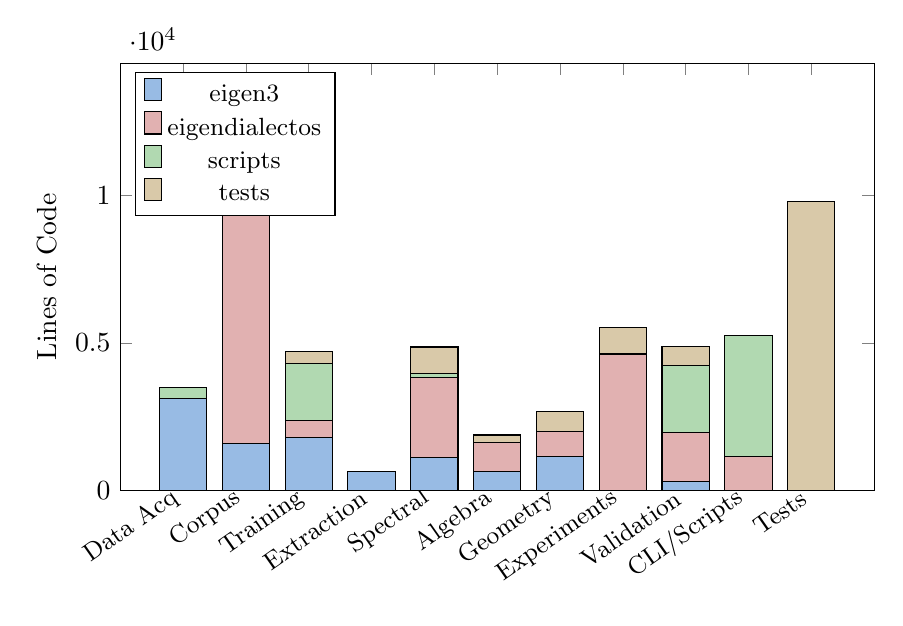
\begin{tikzpicture}
\begin{axis}[
    ybar stacked,
    width=0.92\textwidth,
    height=7cm,
    ylabel={Lines of Code},
    symbolic x coords={
        Data Acq, Corpus, Training, Extraction,
        Spectral, Algebra, Geometry, Experiments,
        Validation, CLI/Scripts, Tests
    },
    xtick=data,
    x tick label style={rotate=35, anchor=east, font=\small},
    legend style={at={(0.02,0.98)},anchor=north west,font=\small},
    ymin=0,
    bar width=0.6cm,
]
\addplot[fill=eigen3col!50] coordinates {
    (Data Acq,3108) (Corpus,1571) (Training,1797) (Extraction,638)
    (Spectral,1124) (Algebra,639) (Geometry,1155) (Experiments,0)
    (Validation,306) (CLI/Scripts,0) (Tests,0)
};
\addlegendentry{eigen3}
\addplot[fill=edcol!40] coordinates {
    (Data Acq,0) (Corpus,9842) (Training,556) (Extraction,0)
    (Spectral,2698) (Algebra,975) (Geometry,846) (Experiments,4625)
    (Validation,1639) (CLI/Scripts,1154) (Tests,0)
};
\addlegendentry{eigendialectos}
\addplot[fill=scriptcol!40] coordinates {
    (Data Acq,392) (Corpus,503) (Training,1957) (Extraction,0)
    (Spectral,138) (Algebra,0) (Geometry,0) (Experiments,0)
    (Validation,2281) (CLI/Scripts,4111) (Tests,0)
};
\addlegendentry{scripts}
\addplot[fill=testcol!40] coordinates {
    (Data Acq,0) (Corpus,1254) (Training,414) (Extraction,0)
    (Spectral,903) (Algebra,260) (Geometry,672) (Experiments,891)
    (Validation,667) (CLI/Scripts,0) (Tests,9813)
};
\addlegendentry{tests}
\end{axis}
\end{tikzpicture}
\caption{LOC distribution by functional area and source package.}
\end{figure}


% ══════════════════════════════════════════════════════════════════════
\section{Architectural Observations}
% ══════════════════════════════════════════════════════════════════════

\begin{enumerate}
  \item \textbf{Dual codebase (\texttt{eigen3} + \texttt{eigendialectos}).}
    The project evolved from a monolithic \texttt{eigen3} package (v1/v3) to a
    modular \texttt{eigendialectos} package (v2). Both coexist, with \texttt{eigen3}
    serving as the active training pipeline and \texttt{eigendialectos} providing
    the expanded corpus, experiment, and validation infrastructure. The downstream
    spectral analysis code is shared.

  \item \textbf{Dimension-agnostic analysis pipeline.}
    All spectral, algebraic, and geometric code operates on arbitrary-dimension
    matrices via NumPy. Changing the embedding dimension (256$\to$384) required
    zero changes outside the training subsystem.

  \item \textbf{Legacy compatibility.}
    Both the transformer and skip-gram training paths are maintained. The
    \texttt{DCLModel}, \texttt{DCLTrainer}, \texttt{SubwordDCLDataset},
    \texttt{DialectContrastiveLoss}, and \texttt{SubwordToWordComposer} classes
    are kept byte-identical for backward compatibility.

  \item \textbf{Data acquisition is the largest component.}
    3{,}108 LOC in \texttt{eigen3} + 9{,}842 LOC in \texttt{eigendialectos}
    devoted to corpus acquisition --- reflecting the reality that obtaining
    balanced, representative dialectal text is the project's primary bottleneck.

  \item \textbf{Test gap in training subsystem.}
    The v2 transformer training machinery (\texttt{TransformerTrainer}, SupCon loss,
    \texttt{BalancedVarietySampler}, XBM queue) has no dedicated unit tests. All 742
    passing tests cover the downstream analysis pipeline. This is the most
    significant quality risk in the current codebase.

  \item \textbf{Experiment richness.}
    13 named experiments spanning spectral topology, phase transitions, impossible
    dialects, cross-linguistic transfer, and code-switching represent a mature
    research framework. The spectral algebra enables novel computational
    dialectology experiments not possible with standard NLP approaches.
\end{enumerate}

\vspace{1em}
\hrule
\vspace{0.5em}
{\small\textit{End of report. Generated for EigenDialectos software architecture review, April 2026.}}

\end{document}
